%%%%%%%%%%%%%%%%%%%%%%%%%%%%%%%%%%%%%%%%%
% Beamer Presentation
% LaTeX Template
% Version 1.0 (10/11/12)
%
% This template has been downloaded from:
% http://www.LaTeXTemplates.com
%
% License:
% CC BY-NC-SA 3.0 (http://creativecommons.org/licenses/by-nc-sa/3.0/)
%
%%%%%%%%%%%%%%%%%%%%%%%%%%%%%%%%%%%%%%%%%

%----------------------------------------------------------------------------------------
%	PACKAGES AND THEMES
%----------------------------------------------------------------------------------------

\documentclass{beamer}

\mode<presentation> {

% The Beamer class comes with a number of default slide themes
% which change the colors and layouts of slides. Below this is a list
% of all the themes, uncomment each in turn to see what they look like.

%\usetheme{default}
%\usetheme{AnnArbor}
%\usetheme{Antibes}
%\usetheme{Bergen}
%\usetheme{Berkeley}
%\usetheme{Berlin}
%\usetheme{Boadilla}
%\usetheme{CambridgeUS}
%\usetheme{Copenhagen}
%\usetheme{Darmstadt}
%\usetheme{Dresden}
%\usetheme{Frankfurt}
%\usetheme{Goettingen}
%\usetheme{Hannover}
%\usetheme{Ilmenau}
%\usetheme{JuanLesPins}
%\usetheme{Luebeck}
\usetheme{Madrid}
%\usetheme{Malmoe}
%\usetheme{Marburg}
%\usetheme{Montpellier}
%\usetheme{PaloAlto}
%\usetheme{Pittsburgh}
%\usetheme{Rochester}
%\usetheme{Singapore}
%\usetheme{Szeged}
%\usetheme{Warsaw}

% As well as themes, the Beamer class has a number of color themes
% for any slide theme. Uncomment each of these in turn to see how it
% changes the colors of your current slide theme.

%\usecolortheme{albatross}
%\usecolortheme{beaver}
%\usecolortheme{beetle}
%\usecolortheme{crane}
%\usecolortheme{dolphin}
%\usecolortheme{dove}
%\usecolortheme{fly}
%\usecolortheme{lily}
%\usecolortheme{orchid}
%\usecolortheme{rose}
%\usecolortheme{seagull}
%\usecolortheme{seahorse}
%\usecolortheme{whale}
%\usecolortheme{wolverine}

%\setbeamertemplate{footline} % To remove the footer line in all slides uncomment this line
%\setbeamertemplate{footline}[page number] % To replace the footer line in all slides with a simple slide count uncomment this line

%\setbeamertemplate{navigation symbols}{} % To remove the navigation symbols from the bottom of all slides uncomment this line
}

\usepackage{graphicx} % Allows including images
\usepackage{booktabs} % Allows the use of \toprule, \midrule and \bottomrule in tables

%----------------------------------------------------------------------------------------
%	TITLE PAGE
%----------------------------------------------------------------------------------------

\title[Sparse DFT recovery]{Sparse DFT recovery via $l_1$ constraint optimization } % The short title appears at the bottom of every slide, the full title is only on the title page

\author{Wei Kuang} % Your name
\institute[UChicago] % Your institution as it will appear on the bottom of every slide, may be shorthand to save space
{
Department of Statistics, University of Chicago \\ % Your institution for the title page
\medskip
\textit{weikuang@uchicago.edu} % Your email address
}
\date{\today} % Date, can be changed to a custom date

\begin{document}

%\begin{frame}
%\titlepage % Print the title page as the first slide
%\end{frame}

%\begin{frame}
%\frametitle{Overview} % Table of contents slide, comment this block out to remove it
%\tableofcontents % Throughout your presentation, if you choose to use \section{} and \subsection{} commands, these will automatically be printed on this slide as an overview of your presentation
%\end{frame}

%----------------------------------------------------------------------------------------
%	PRESENTATION SLIDES
%----------------------------------------------------------------------------------------


%------------------------------------------------
\section{Problem Formulation} % Sections can be created in order to organize your presentation into discrete blocks, all sections and subsections are automatically printed in the table of contents as an overview of the talk
%------------------------------------------------

%\subsection{Subsection Example} % A subsection can be created just before a set of slides with a common theme to further break down your presentation into chunks
\begin{frame}
\frametitle{Log-barrier method}
Consider the optimization problem
\begin{equation}
    min_x f(x)\text{ s.t. }c(x)\leq 0
\end{equation}
E.g. $min_x \|y-X \beta\| \text{ s.t. } \|\beta\|_1\leq d$
\begin{itemize}
    \item Add a penality term: 
    $$\min_x f(x)+\lambda c(x)$$
    (the problem formulation for ADMM)
    \item Log barrier method: 
    $$\min_x f(x)+I_{-}(c(x))$$
    where
    $$
    I_{-}(u) = 0 \text{ if } u\leq 0, \text{ otherwise }I_{-}(u)=\infty
    $$
\end{itemize}
\end{frame}

\begin{frame}
\frametitle{Log-barrier method}
\begin{itemize}
    \item Log barrier method: 
    $$\min_x f(x)+I_{-}(c(x))$$
    $I_{-}(c(x))$ is not differentialable
    \item Approaching $I_{-}(u)$ as $t$ goes to infinity
    $$
    \min_x f(x)-\frac{1}{t}log(-c(x))
    $$
\end{itemize}
\begin{figure}
    \centering
    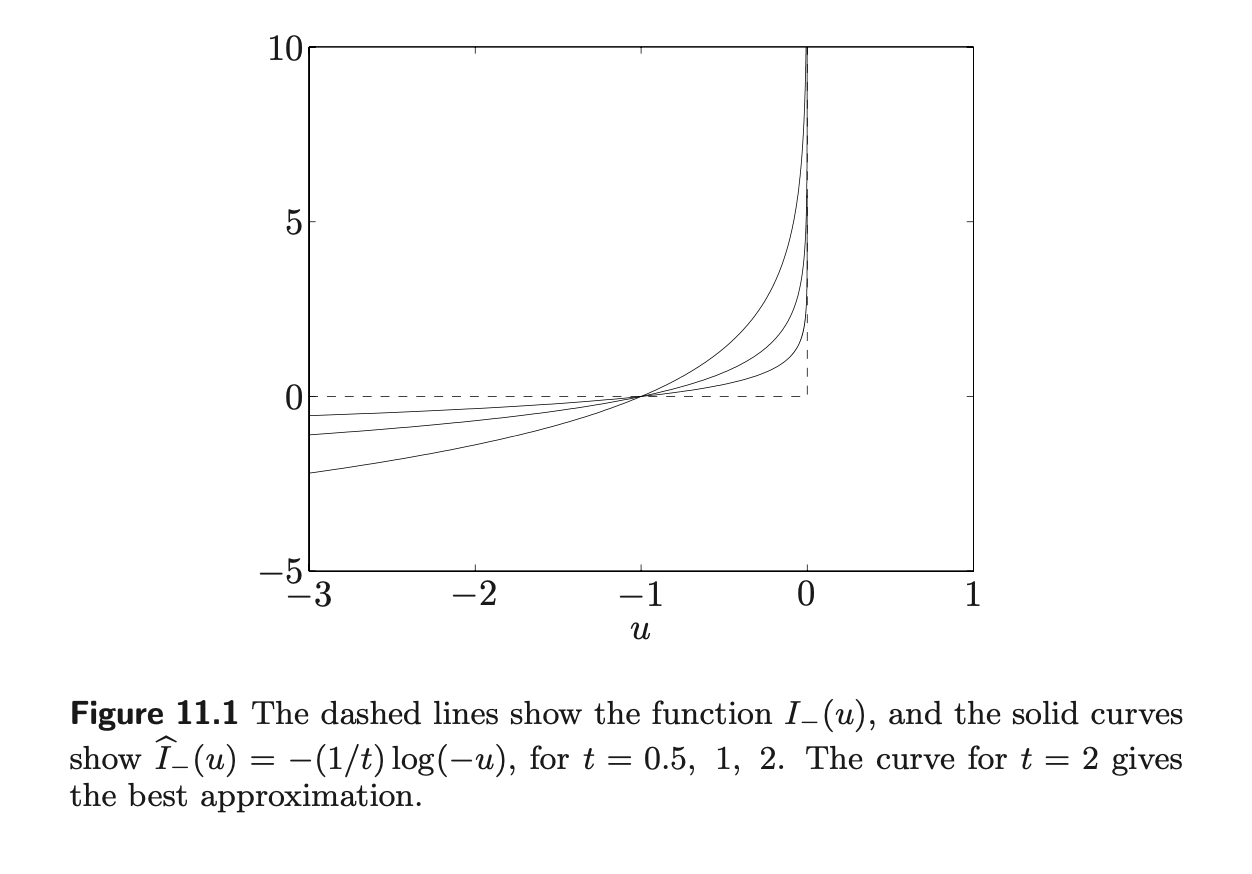
\includegraphics[width=0.6\linewidth]{Interior Point Method/logbarrier.png}
    %\caption{Caption}
    %\label{fig:enter-label}
\end{figure}
\end{frame}

\begin{frame}{Newton system}
    \begin{itemize}
        \item Solve the Newton system $\nabla^2 \psi \Delta x = -\nabla \psi$
        \item $\Delta x = -\left(\nabla^2 \psi\right)^{-1}\nabla \psi$
        \begin{itemize}
            \item use Shermon-Morrison formula to explicitly compute $\left(\nabla^2 \psi\right)^{-1}$
            \item computational complexity is $O(nm)+O(m^3)$
            \item storage: generate matrix $M$ with size $m\times n$
        \end{itemize}
    \item use Conjugate gradient method to approximately solve the system
    \begin{itemize}
        \item within each iteration: only involves matrix-vector product
        \item matrix-free: not need to store M
        \item numbers of CG iterations are reasonable
    \end{itemize}
    \end{itemize}
\end{frame}

\begin{frame}{Numerical result}
\begin{figure}
    \centering
    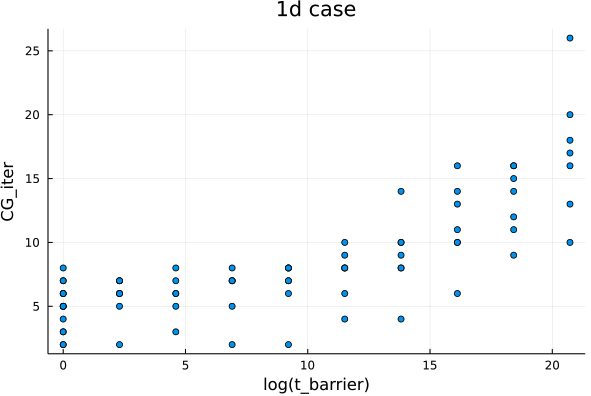
\includegraphics[width=0.6\linewidth]{Interior Point Method/1d_missing.png}
    %\caption{Caption}
    %\label{fig:enter-label}
\end{figure}
\end{frame}

\begin{frame}{Numerical result}
\begin{figure}
    \centering
    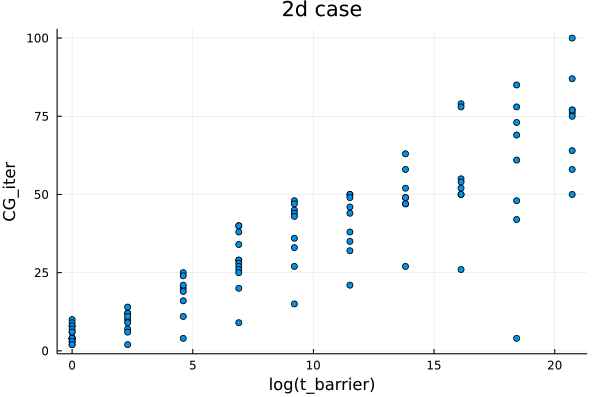
\includegraphics[width=0.6\linewidth]{Interior Point Method/2d_missing.png}
    %\caption{Caption}
    %\label{fig:enter-label}
\end{figure}
\end{frame}

\begin{frame}{Numerical result}
\begin{figure}
    \centering
    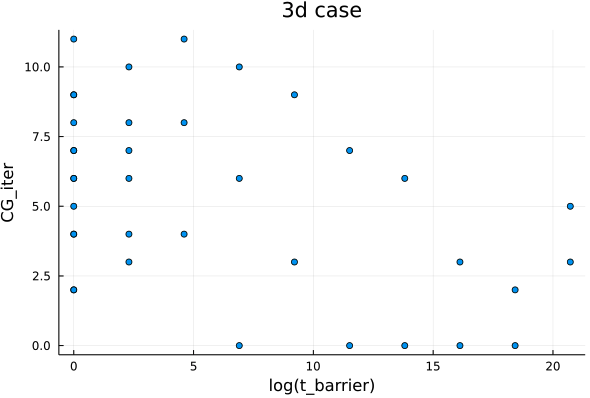
\includegraphics[width=0.6\linewidth]{Interior Point Method/3d_missing.png}
    %\caption{Caption}
    %\label{fig:enter-label}
\end{figure}
\end{frame}


\begin{frame}{Numerical result}
\begin{figure}
    \centering
    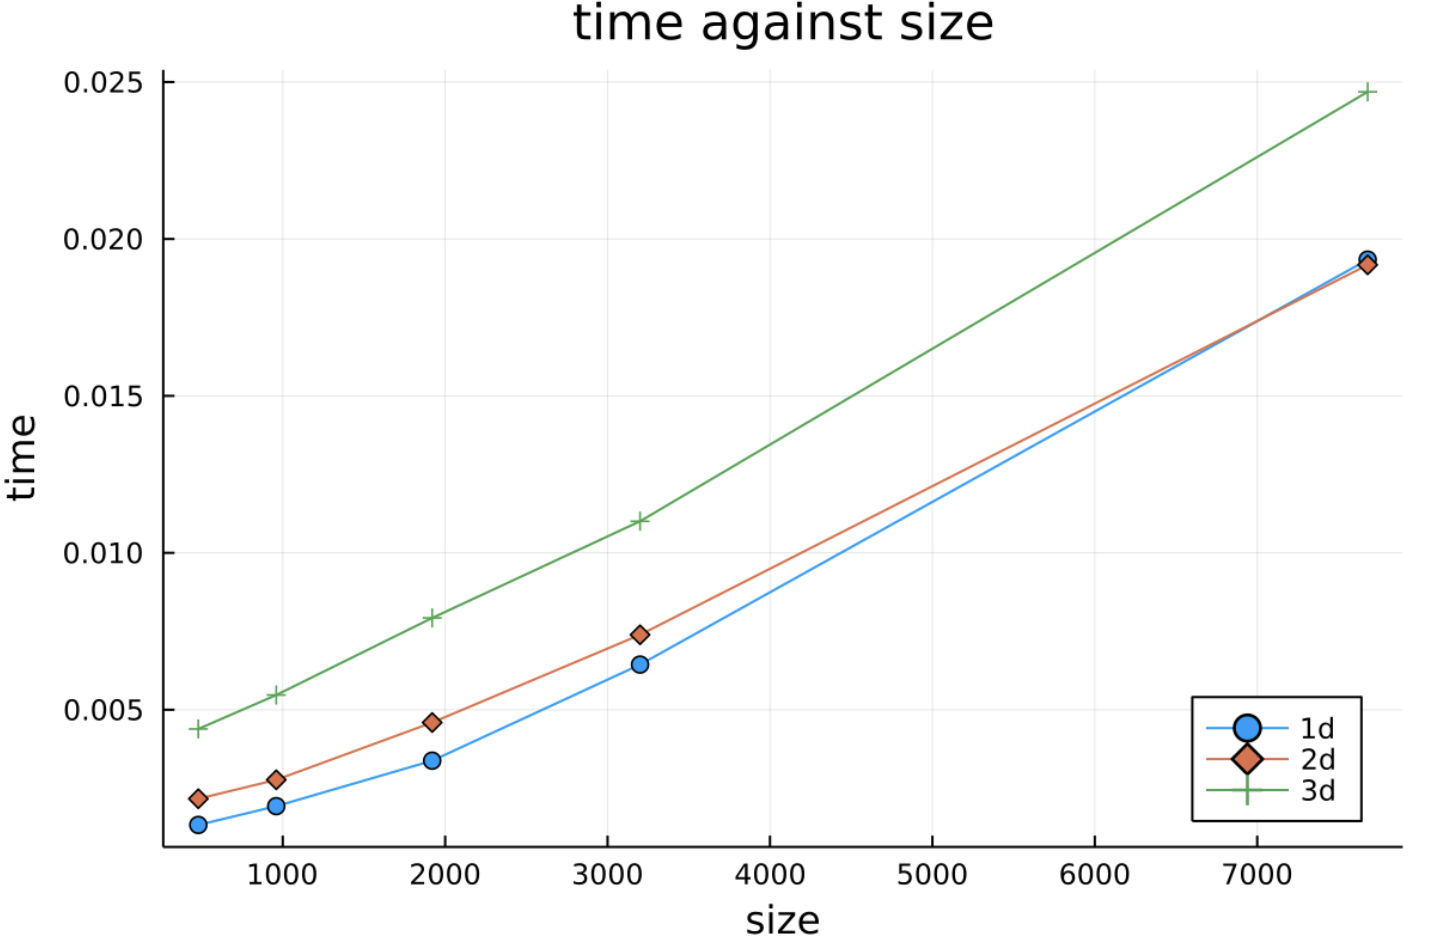
\includegraphics[width=0.6\linewidth]{Interior Point Method/time against size.png}
    %\caption{Caption}
    %\label{fig:enter-label}
\end{figure}
\end{frame}

%------------------------------------------------

\begin{frame}
\frametitle{References}
\footnotesize{
\begin{thebibliography}{99} % Beamer does not support BibTeX so references must be inserted manually as below
\bibitem[Hassanieh, 2012]{p1} Hassanieh, Haitham and Indyk, Piotr and Katabi, Dina and Price, Eric (2012)
\newblock Simple and practical algorithm for sparse Fourier transform
\newblock \emph{Proceedings of the twenty-third annual ACM-SIAM symposium on Discrete Algorithms} 1183--1194.

\bibitem[Tibshirani, 1996]{p2} Tibshirani, Robert (1996)
\newblock Regression shrinkage and selection via the lasso
\newblock \emph{Journal of the Royal Statistical Society: Series B (Methodological)} 58(1) 267--288.

\bibitem[Boyd, 2004]{p3} Boyd, Stephen and Boyd, Stephen P and Vandenberghe, Lieven (2004)
\newblock Convex optimization
\newblock \emph{Cambridge university press}
\end{thebibliography}
}
\end{frame}

%------------------------------------------------

\begin{frame}
\Huge{\centerline{The End}}
\end{frame}

%----------------------------------------------------------------------------------------

\end{document}